Στην τελευεταία άσκηση του παραδοτέου ζητείται να συνδυάσουμε όλα τα προηγούμενα $modules$
και να υλοποιήσουμε τον $RISC-V$ επεξεργαστή μας. Σε 
\\
Οι εντολές που μπορούμε να αποσπάσουμε από το αρχείο $rom\_bytes.v$, όταν λαμβάνουμε ως
μια εντολή κάθε τέσσερις γραμμές, είναι:
\selectlanguage{english}
\begin{minted}{verilog}
    addi x1, x0, 7
    addi x2, x0, 21
    add x3, x1, x2
    addi x4, x0, -9
    addi x5, x2, -17
    add x6, x5, x4
    sub x7, x3, x2
    sll x8, x7, x5
    slt x9, x4, x8
    xor x10, x8, x2
    and x11, x10, x8
    srl x12, x11, x9
    or x13, x12, x3
    sra x14, x4, x9
    sw x11, 0(x5)
    lw x15, 0(x5)
    andi x16, x8, -45
    ori x17, x16, 22
    srli x18, x13, 1
    beq x15, x11, 16
    // 4 blank instructions
    slti x9, x18, 15
    xori x19, x8, 58
    slli x20, x17, 1
    srai x5, x15, 2
    // 100 blank instructions
\end{minted}
\selectlanguage{greek}Σχηματικό διάγραμμα από το $FSM$:
\begin{figure}[H]
    \centering
    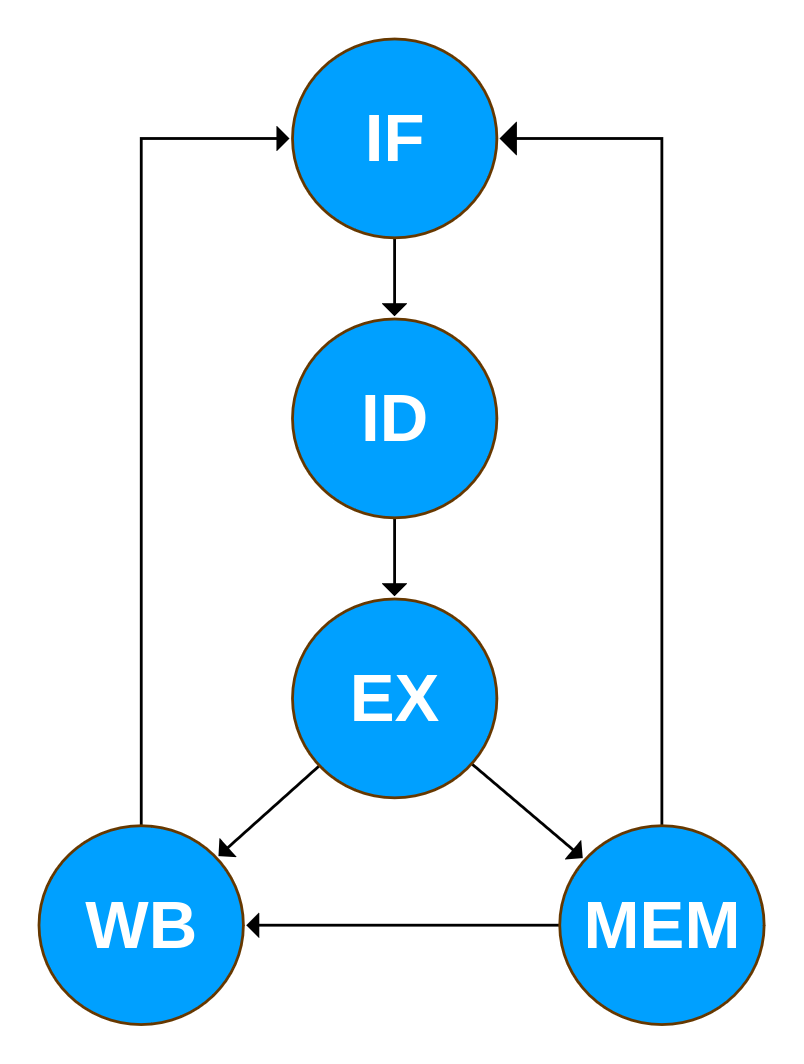
\includegraphics[width=0.6\textwidth]{media/exercise5_fsm.png}
    \caption{Σχηματικό διάγραμμα $FSM$}
\end{figure}
Κυματομορφές προσομοίωσης:
% \begin{figure}[H]
%     \centering
%     \includegraphics[width=1\textwidth]{media/exercise5_waveforms.png}
% \end{figure}